  \chapter{Introducción}
Este proyecto dispone del código fuente, ejemplos y procedimientos de instalación en un \href{https://github.com/andrelorenzo/Vision2D_navigation}{repositorio} público de GitHub.

Uno de los principales retos actualmente en la navegación de UAVs es la evitación de obstáculos. La mayoría de los drones no cuentan con sistemas como LiDAR, cámaras 3D (RGB-D) o sonar, principalmente debido a limitaciones de peso, coste o capacidad de procesamiento a bordo, a diferencia de los vehículos terrestres autónomos. Estas limitaciones se agravan aún más en el caso de drones de bajo coste, cada vez más populares para la creación de enjambres o ''swarms''.

    \section{Motivación}
La idea de conseguir un sistema en tiempo real que sea capaz de maniobrar en un espacio obstaculizado sin necesidad de costosos sensores y complejos algoritmos suena interesante, por ello este trabajo de investigación trata de dar solución a este claro problema contando exclusivamente con una cámara de baja resolución RGB. En concreto, se plantea el reto de identificar obstáculos y generar rutas alternativas en tiempo real empleando solo una cámara RGB, sin información explícita de profundidad ni sensores adicionales.

Esta aproximación no solo abre la puerta a soluciones más económicas y ligeras, sino que también plantea nuevas posibilidades para aplicaciones donde el tamaño, el peso o la disponibilidad energética del dron son factores críticos. Desde misiones de exploración en interiores hasta operaciones de reconocimiento en entornos no estructurados, un sistema de navegación visual basado en una única cámara puede ofrecer ventajas significativas si se logra extraer información suficiente del entorno a partir de las imágenes.

Entre los distintos estimadores de profundidad monocular disponibles, el modelo MiDaS destaca especialmente por su equilibrio entre precisión y velocidad. Este estimador se basa en arquitecturas modernas como Vision Transformers (ViTs), que permiten capturar relaciones espaciales globales dentro de la imagen con gran eficiencia. En particular, las versiones ligeras de MiDaS, como MiDaS v2.1 small o las variantes con ViT-S, han sido optimizadas para funcionar en tiempo real incluso en sistemas con recursos limitados, lo que las convierte en candidatas ideales para su uso embarcado o en aplicaciones donde la latencia es crítica.

Gracias a esta arquitectura, MiDaS puede generar mapas de profundidad coherentes y densos a partir de una única imagen RGB, permitiendo extraer información estructural del entorno sin necesidad de sensores físicos adicionales. Esta capacidad, unida a su rendimiento en escenarios no estructurados y su generalización a distintas condiciones de iluminación o texturas, lo convierte en una herramienta esencial dentro de este trabajo, facilitando la navegación visual autónoma en drones ligeros y de bajo coste.

    \section{Herramientas utilizadas}
En este proyecto, la principal preocupación ha sido la velocidad de procesamiento de imágenes, tanto en el envío de estas al ordenador como en las fases de inferencia y procesamiento previas y posteriores a dicha inferencia. En este apartado se describen las herramientas utilizadas, incluyendo los lenguajes, plataformas, librerías y versiones correspondientes.

El código se ha desarrollado en C++ (estándar C++20) y se ejecuta en un sistema Linux Ubuntu 22.04 LTS. Para la inferencia de modelos se ha empleado la versión 2.7 de LibTorch (la versión nativa de PyTorch en C++), con aceleración por CUDA 12.1. Además, se ha utilizado OpenCV 4.12, compilado específicamente para soportar aceleración mediante cuDNN y CUDA.

El hardware utilizado incluye un procesador Intel(R) Core(TM) i5-1035G1 CPU @ 1.00GHz con 8 núcleos, junto con una GPU GeForce MX110.

En el lado del dron, se emplea una cámara ESP32-CAM con una resolución de 640x480 px (VGA), la cual dispone de conectividad Wi-Fi para la transmisión de datos al ordenador de procesamiento en tierra.

  \chapter{Desarrollo}
En el presente capítulo se expone el desarrollo de las distintas implementaciones evaluadas. Dada la naturaleza investigadora de este proyecto, la arquitectura, al igual que el resto de componentes del trabajo, ha sido desarrollada en múltiples variantes tanto a nivel de software como de hardware, con el objetivo de probar distintas aproximaciones y determinar cuál ofrece la mejor solución al problema planteado.
    \section{Arquitectura de la comunicación}
La arquitectura del sistema se divide en 2 secciones, la comunicación entre la cámara (esp32) y el ordenador central, y por otro lado, la arquitectura software de procesamiento de las imágenes tanto en el código de la cámara como en el ordenador principal.

      \subsection{Protocolos y Hardware}
La comunicación es uno de los aspectos clave en este proyecto por dos razones principales. En primer lugar, un mal planteamiento en esta etapa puede generar un cuello de botella que limite la velocidad a la que es posible procesar los fotogramas. En segundo lugar, se trata de la primera etapa de toda la implementación, y por tanto constituye la base sobre la que se apoyará el resto del sistema. Por esta razón, se han desarrollado y probado dos métodos de comunicación:

El primero se basa en la incorporación de un tercer dispositivo (ESP32 master) que actúa como bridge entre la cámara y el ordenador. Esta estrategia se eligió dado que el protocolo \textbf{espnow} ofrece una distancia máxima de hasta 480 m, lo que favorece la comunicación con el dron desde tierra. Además, este protocolo destaca por su baja latencia, lo que resulta especialmente ventajoso en aplicaciones en tiempo real. El esquema de esta arquitectura se muestra en la~\textbf{figura \ref{fig:comms_esquema_espnow}}.

\vspace{1cm}
\begin{figure}[H] % Usa [H] si quieres que quede exactamente en ese lugar (requiere \usepackage{float})
    \centering
    \begin{tikzpicture}[>=Latex, node distance=4cm, every node/.style={font=\small}]

    % Nodos
    \node[draw, rectangle, rounded corners, minimum width=2.5cm, minimum height=1.2cm, align=center] (esp_cam) {ESP CAM};
    \node[draw, rectangle, rounded corners, minimum width=2.5cm, minimum height=1.2cm, align=center, right=of esp_cam] (esp_master) {ESP master};
    \node[draw, rectangle, rounded corners, minimum width=2.5cm, minimum height=1.2cm, align=center, right=of esp_master] (pc) {PC};

    % Flechas bidireccionales
    \draw[<->] (esp_cam) -- node[above]{\textbf{ESP-NOW}} (esp_master);
    \draw[<->] (esp_master) -- node[above]{\textbf{Serial}} (pc);

    \end{tikzpicture}
    \caption{Esquema de comunicación entre módulos: ESP CAM, ESP master y PC mediante protocolo espnow.}
    \label{fig:comms_esquema_espnow}
\end{figure}


El segundo esquema de comunicación es más sencillo y se compone únicamente de la cámara y el ordenador. En este caso, la comunicación se realiza mediante Wi-Fi, utilizando el protocolo TCP para garantizar la correcta recepción de los datos. Esta configuración se muestra en la~\textbf{figura~\ref{fig:comms_esquema_wifi}}.

\vspace{1cm}
\begin{figure}[H] % Usa [H] si quieres que quede exactamente en ese lugar (requiere \usepackage{float})
    \centering
    \begin{tikzpicture}[>=Latex, node distance=4cm, every node/.style={font=\small}]

    % Nodos
    \node[draw, rectangle, rounded corners, minimum width=2.5cm, minimum height=1.2cm, align=center] (esp_cam) {ESP CAM};
    \node[draw, rectangle, rounded corners, minimum width=2.5cm, minimum height=1.2cm, align=center, right=of esp_master] (pc) {PC};

    % Flechas bidireccionales
    \draw[<->] (esp_cam) -- node[above]{\textbf{WIFI (TCP)}} (pc);

    \end{tikzpicture}
    \caption{Esquema de comunicación entre módulos: ESP CAM y PC mediante Wifi 2.4 Ghz.}
    \label{fig:comms_esquema_wifi}
\end{figure}

En la \textbf{tabla \ref{tab:comp_now_wifi}} se muestran las diferencias entre los dos protocolos, cuales son sus ventajas y desventajas. Como se puede observar, el protocolo espnow parace ser perfecto para la tarea, sobre todo por el rango y la baja latencia, por ello esta fue la primera arquitectura que se probó.

\begin{table}[H]
    \centering
    \begin{tabular}{|c|c|c|}
        \hline
        \textbf{Especificación} & \textbf{ESPNOW} & \textbf{WIFI (TCP)} \\
        \hline
        Frecuencia      & 2.4 GHz & 2.4 GHz \\
        Velocidad       & 200 - 300 Kbps & 1 - 10 Mbps \\
        Latencia        & 2 - 5 ms & 10 - 100 ms\\
        Consumo         & Bajo & Medio \\
        Fiabilidad      & Nula & Muy Alta\\
        Compatibilidad  & solo esp32 & Muy alta\\
        Rango           & $<$ 480 m & $<$ 300 m\\
        Tamaño del paquete & 250 bytes & 2500 bytes \\
        \hline
    \end{tabular}
    \caption{Comparación de especificaciones entre protocolos de comunicación.}
    \label{tab:comp_now_wifi}
\end{table}
      \subsection{Software}



El flujo de operación para la arquitectura nº 1 (\textit{espnow}) se basa en dos bucles de comunicación. En el primero, la cámara y el \textit{esp32-master} intercambian los fotogramas capturados por la cámara a la máxima velocidad que esta permite. El proceso consiste en capturar la imagen, dividirla en n paquetes de 200 bytes cada uno (reservando 50 bytes para un posible envío de telemetría), y enviarlos mediante \textit{espnow}. A cada imagen se le añaden los siguientes campos: un identificador de paquete, el número total de paquetes y el tamaño total de la imagen en bytes, con el siguiente formato:

\textbf{$$[id][n][size][img]$$}

En el lado receptor, el \textit{esp32-master} va recibiendo los paquetes hasta completar la imagen. A continuación, verifica si se ha perdido alguno; en caso afirmativo, solicita a la cámara el reenvío del paquete faltante, indicando su identificador correspondiente.

Para esta arquitectura, la cámara captura imágenes con una resolución de 320x240x3 px y las comprime en \textbf{JPEG} con una calidad de 10. El tamaño medio resultante es de aproximadamente 8000 bytes, lo que equivale a unos 40 paquetes por imagen. Estas imágenes se almacenan temporalmente en la memoria flash (SPIFFS) del \textit{esp32-master}, que actúa como búfer intermedio.

Posteriormente, el segundo bucle de comunicación se establece entre el \textit{esp32-master} y el ordenador, donde la imagen \textbf{JPEG} se serializa y se transmite por puerto serie a la máxima velocidad soportada por el sistema, en este caso 250000 baudios.

Los resultados obtenidos para la mejor versión de este algoritmo (sin realizar ninguna operación matemática en el ordenador, únicamente mostrando la imagen con OpenCV) alcanzan una velocidad de entre \textbf{0.5 y 1.5 fps}. No obstante, una proporción significativa de los fotogramas llega corrupta, a pesar de haberse implementado mecanismos de aseguramiento de entrega de paquetes.

En el caso de la arquitectura nº 2, el procedimiento es considerablemente más sencillo. La cámara genera una red Wi-Fi a la que el ordenador se conecta directamente, estableciendo una comunicación punto a punto fiable. Gracias a la mayor velocidad de transmisión que ofrece esta interfaz, los resultados son significativamente más prometedores, alcanzando una velocidad de recepción de entre \textbf{30 y 40 fps}, con imágenes de 640x480x3 px comprimidas en \textbf{JPEG} con una calidad de 15 y sin pérdida de datos, gracias al uso del protocolo TCP.

A causa de la baja velocidad de transmisión en la comunicación por espnow, se escogió la arquitectura nº 2 como base para el resto del proyecto.

    \section{Modelos para inferencia de datos}
Al llegar a esta parte del proyecto se desarrolló una investigación sobre las principales implementaciones de estimación de profundidad, entre muchos modelos destaca \textit{MiDaS v2.1} por su rapidez y \textit{depth anything v2} por su estabilidad y precisión. Los dataset con los que han sido entrenados también son un punto extremadamente importante a la hora de escoger el modelo, en este caso destacan \textbf{KITTY y cityscapes}, 2 datasets de todo tipo de sensores 3D en exteriores.
Otro punto importante que se ha buscado en todo momento es que el modelo exista o se pueda crear en formato onnx (Open Neural Network Exchange), este es un formato estandarizado que solo cuenta con funciones simples y que promete hacer más rápida la inferencia de los datos, por otro lado, esto también limita la búsqueda a causa de que no todos los modelos son convertibles a onnx y la conversión para los que si lo son no es trivial.

        \subsection{Estimadores de profundidad}
En la \textbf{tabla \ref{tab:mercado_estudio}} se muestra un pequeño análisis de ''mercado'' sobre los modelos que existen junto con sus puntos fuertes, en la \textbf{tabla \ref{tab:estudio_fps}} se muestran los modelos que se pudieron transformar o conseguir en onnx y por tanto ser probados para así, comprobar su tiempo de inferencia en el código.


\begin{table}[h]
    \centering
    \begin{tabular}{|c|c|c|c|}
        \hline
        \textbf{Modelo} & \textbf{Velocidad}    & \textbf{Precisión}    & \textbf{Consistencia}   \\
        \hline
        MiDaS v21           & Muy alta          & Baja                  & Baja                      \\
        MiDaS v30           & Baja              & Alta                  & Media                     \\
        Depth anything v2   & Media             & Media                 & Media                     \\
        Depth pro           & Muy baja          & Muy Alta              & Alta                      \\
        Marigold            & Baja              & Alta                  & Media                      \\
        DepthCrafter        & Muy baja          & Alta                  & Muy alta                  \\
        Metric3D            & baja              & Muy alta              & Alta                      \\
        \hline
    \end{tabular}
    \caption{Comparación de las características de los modelos más populares hoy en día.}
    \label{tab:mercado_estudio}
\end{table}


\begin{table}[h]
    \centering
    \begin{tabular}{|c|c|c|c|}
        \hline
        \textbf{Modelo} & \textbf{tiempo (ms)}    & \textbf{fps}    \\
        \hline
        MiDaS v21 small             & 97.26             & 10.28              \\
        MiDaS v21 medium            & 866.23          & 1.15              \\
        MiDaS v30 hybrid            & 1279.50            & 0.78             \\
        Depth anything v1.0         & 473.93           & 2.11               \\
        Depth anything v2.0         & 563.66            & 1.77              \\
        Depth anything outdoors     & 813.00          & 1.23              \\
        \hline
    \end{tabular}
    \caption{Comparación de los modelos prometedores para ser usados.}
    \label{tab:estudio_fps}
\end{table}


Al realizar las pruebas se obtuvo una conclusión clara, el único modelo viable para el proyecto es el \textit{MiDaS small v2.1} y el modelo \textit{depth Anything v1.0} como opción B. Tanto el modelo MiDaS como el depth anything son modelos que sacan un mapa de profundidad relativo a los objetos que ven, es decir lo que te muestran es la diferencia de profundidad en una escala desde 0 (lo más profundo) hasta 1200 (lo más cercano) en valores enteros. En el caso de depth anything el rango es de 0 a 5 pero con valores decimales. En las \textbf{figuras \ref{fig:midas_test} y \ref{fig:depth_Any_test}} se puede observar los valores de la distancia relativa que saca el modelo.


\begin{figure}[H]
    \centering
    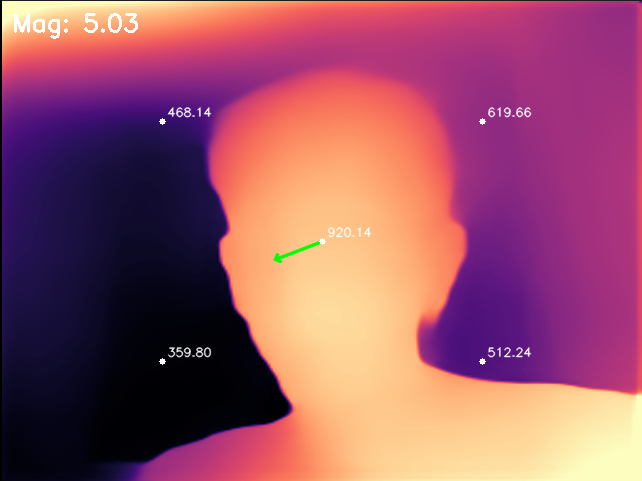
\includegraphics[width=0.8\textwidth]{images/midas_test.png}
    \caption{Salida de MiDaS v21 small.}
    \label{fig:midas_test}
\end{figure}

\begin{figure}[H]
    \centering
    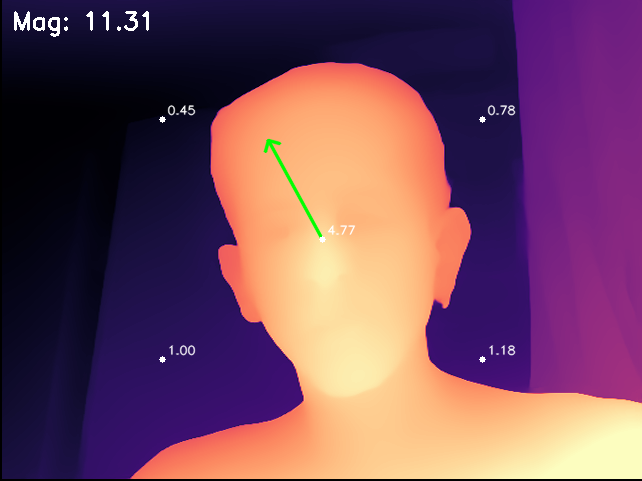
\includegraphics[width=0.8\textwidth]{images/depth_any_test.png}
    \caption{Salida de depth anything v1.0.}
    \label{fig:depth_Any_test}
\end{figure}

        \subsection{Detectores y clasificadores de objetos}
Por otro lado se probaron 2 versiones del modelo nano de \textbf{YOLO} (You Only Look Once), en concreto la version 5 y la 11, ambas entrenadas con \textbf{COCO}, dado que no se notó ninguna gran diferencia en el tiempo de inferencia entre estos 2 modelos se escogió la versión mas moderna, YOLO v11, este modelo es un detector de objetos que servirá para poder extrapolar la distancia del mapa de distancias relativo que sacan los estimadores de profundidad.
    \section{Aceleración y optimización}
Como ya se ha comentado con anterioridad la principal preocupación de este trabajo es conseguir una velocidad suficiente para poder, más adelante realizar algoritmos de visión con un frame rate aceptable. 

        \subsection{Multi-threading}
Por ello, se han añadido diversos métodos de aceleración por hardware que ayudan a maximizar la potencia de computo, para empezar se realizó una estructura multi-threading con 4 threads, cada uno ejecutando una tarea específica:

\begin{enumerate}
    \item \textbf{CAPTURE thread}, este thread se encarga de comandar a la cámara que capture un frame y lo envié al ordenador, este proceso se considera el cuello de botella principal y por tanto da el máximo teórico de fps que se pueden conseguir, con una media de 35,47 ms entre petición y recepción del frame se tienen 28,19 fps.
    \item \textbf{YOLO thread}, este es el encargado de inferir el modelo de YOLO el cual se ejecuta en la CPU. El tiempo de inferencia medio es de 95.905 ms.
    \item \textbf{MIDAS thread}, el thread que ejecuta MiDaS se encarga de inferir el modelo de MiDaS ejecutándolo en la GPU. El tiempo de inferencia medio es de 105.868 ms.
    \item \textbf{MAIN thread}, el thread principal se encarga de coger las salidas de las 2 inferencias y ejecutar los algoritmos de visión que más adelante se explica.
\end{enumerate}

Se podría pensar que ejecutar ambos modelos en la GPU aceleraría el proceso; sin embargo, ocurre lo contrario. Si bien es ampliamente conocido que la inferencia de modelos de inteligencia artificial se beneficia del uso de GPU, en este caso particular, al disponer de una única unidad de procesamiento gráfico, la ejecución concurrente de dos modelos introduce un nuevo cuello de botella. Cada modelo debe esperar a que finalice la inferencia del otro, lo que provoca una ralentización del proceso de hasta un 61 \% (pasando de 140 ms a los ya comentados 105 ms). En la \textbf{figura \ref{fig:midas_yolo_rpfiling}} se puede observar un análisis realizado con MiDaS en la GPU y YOLO en la CPU.


\begin{figure}[htbp]
    \centering
    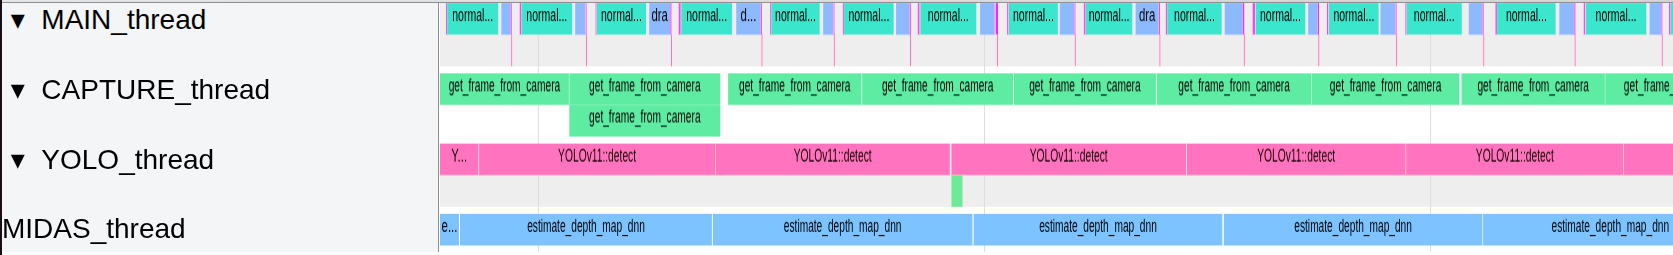
\includegraphics[width=1\textwidth]{images/profiling_midas_yolo.png}
    \caption{Profiling de 5 ciclos de inferencia con MiDaS (GPU) + YOLO v11 (CPU).}
    \label{fig:midas_yolo_rpfiling}
\end{figure}


        \subsection{Aceleración con GPU y CUDA}
Otra aceleración por hardware que se ha implementado es como ya se ha comentado el uso de la GPU para inferir en el modelo más pesado (MiDaS), para ello se ha hecho uso de OpenCV compilado con CUDA, cuDNN y la arquitectura de la GPU de la que se dispone (MX110). Esta implementación supuso una mejora del 32\%.

        \subsection{Uso de modelos simplificados ONNX}
Finalmente, se optó por utilizar exclusivamente modelos en formato ONNX. Esta decisión se basa en varias ventajas clave que ofrece dicho formato. Los modelos ONNX (Open Neural Network Exchange) están diseñados para ser altamente portables y eficientes, lo que facilita su integración en entornos con recursos limitados o donde la velocidad de inferencia es crítica.

Como se ha mencionado previamente, estos modelos suelen estar optimizados mediante técnicas como la cuantización o la eliminación de capas redundantes, lo que reduce significativamente su tamaño y complejidad sin comprometer de forma notable la precisión. Además, ONNX permite una ejecución más ágil gracias a su compatibilidad con motores de inferencia altamente optimizados como ONNX Runtime, TensorRT, OpenVINO o OPenCV, este último es el que se ha utilizado para el proyecto.
    \section{Inferencia de la dirección de movimiento}
El objetivo final del proyecto es, por supuesto, lograr dirigir a un dron en una dirección de libre camino, la primera idea que se te puede venir a la cabeza es posiblemente crear un mapa de obstáculos basándonos en la visión de la cámara, la odometría y GPS del dron, es decir, reaiza un SLAM visual. El problema llega al intentar realizarlo en tiempo real donde lo más probable es que sea tan lento que inviable para su uso. Es por ello, que en el presente trabajo se tomo una dirección diferente, más liviana y por tanto más rápida.

Al observar la imagen de salida que proporciona MiDaS, \textbf{figura \ref{fig:midas_midas}}, podemos observar 2 características clave, la primera es que los puntos más profundos tienen valores más próximos a '0' y los puntos más cercanos tienen valores más altos, además, la diferencia de valores entre 2 puntos es mayor cuanto mayor es la diferencia de profundidad. Si además, se plantea la imagen como una curva continúa en 3 dimensiones se puede ver rapidamente que la dirección de máxima pendiente de esa curva apunta a la zona de la imagen con mayor profundidad, o desde otro punto de vista, la zona con menor densidad de obstaculos cercanos.


\begin{figure}[H]
    \centering
    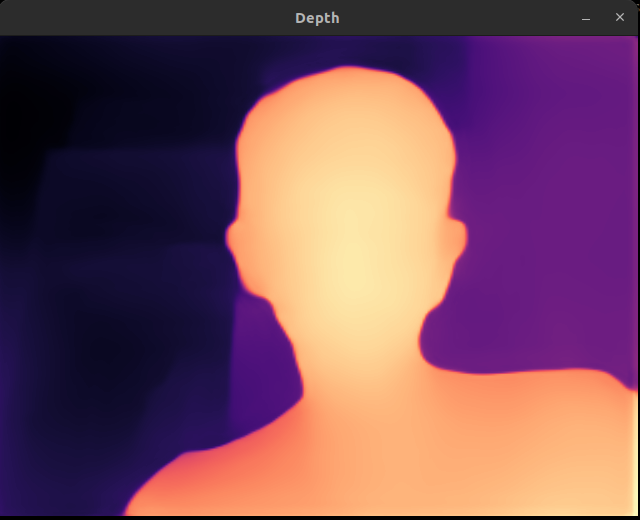
\includegraphics[width=0.7\textwidth]{images/midas_midas.png}
    \caption{Salida de MiDaS sin procesamiento.}
    \label{fig:midas_midas}
\end{figure}


Es por ello que si se aplica el $-\nabla{M}$ donde M es la salida de MiDaS y de todos esos puntos hayamos la media obtenemos un vector que apunta a la zona con menos obstáculos, además cuanta mayor es la diferencia de distancia entre los obstáculos mayor es la magnitud de ese vector, por tanto podemos usar esta dirección y magnitud para comandar al dron hacia una zona segura. En la \textbf{figura \ref{fig:dir_body} y figura \ref{fig:dir_back}} se observa un ejemplo donde el drone tiene varios caminos posibles para evitar al obstaculo, el algoritmo por su naturaleza escogerá el camino con mayor libertad de movimiento, en la \textbf{figura \ref{fig:dir_nomove}} se puede observar un caso en el que el drone no podría esquivar el obstáculo con seguridad por tenerlo muy cerca, en este caso se podría detectar y retroceder para encontrar otro camino, finalmente se observa en la \textbf{figura \ref{fig:dir_wall}} un caso donde aparece un muro cercano en el lado derecho de la imagen y por tanto el algoritmo indica una dirección opuesta con gran magnitud para esquivarlo.


\begin{figure}[h]
    \centering
    \begin{minipage}{0.49\textwidth}
        \centering
        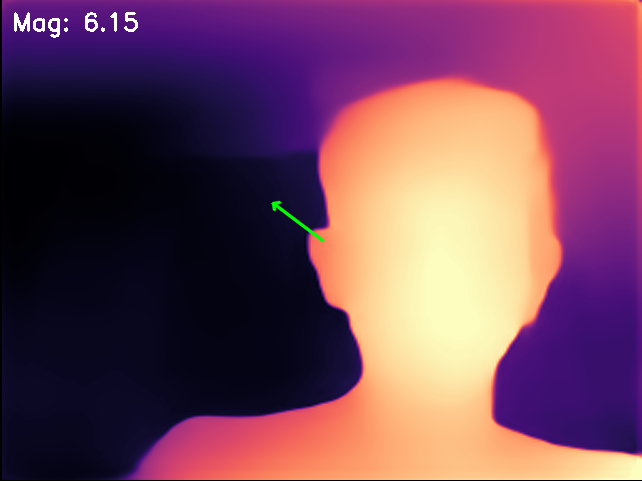
\includegraphics[width=\linewidth]{images/get_dir_body1.png}
        \caption{Dirección con 2 obstaculos con diferente profundidad.}
        \label{fig:dir_body}
    \end{minipage}
    \hfill
    \begin{minipage}{0.49\textwidth}
        \centering
        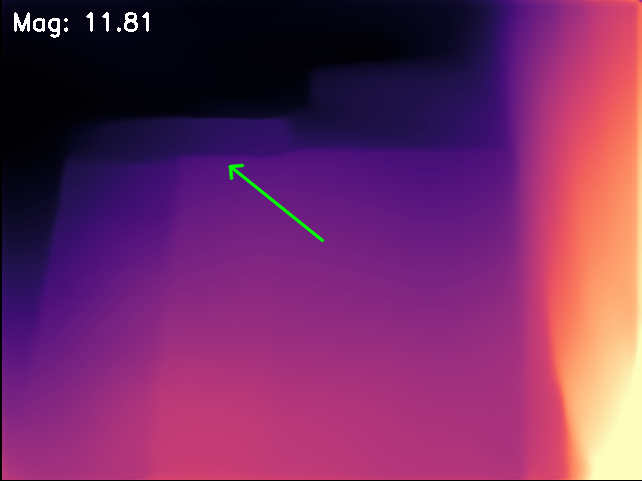
\includegraphics[width=\linewidth]{images/get_dir_background2.png}
        \caption{Dirección con solo 1 obstáculo a una distancia medía}
        \label{fig:dir_back}
    \end{minipage}
    
    \vspace{0.5cm} % Espacio entre filas

    \begin{minipage}{0.49\textwidth}
        \centering
        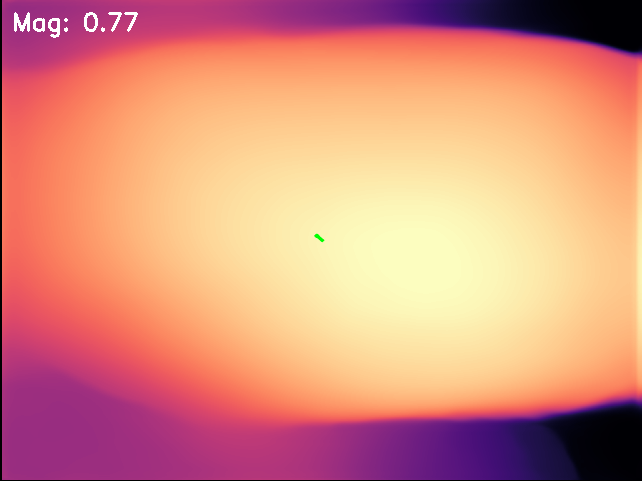
\includegraphics[width=\linewidth]{images/get_dir_nomove3.png}
        \caption{Dirección en una posición sin posibilidad de movimiento.}
        \label{fig:dir_nomove}
    \end{minipage}
    \hfill
    \begin{minipage}{0.49\textwidth}
        \centering
        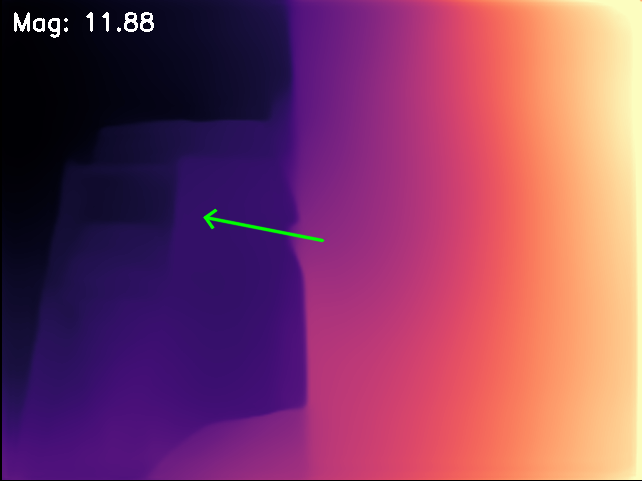
\includegraphics[width=\linewidth]{images/get_dir_wall4.png}
        \caption{Dirección en una posición con el final de un muro cercano.}
        \label{fig:dir_wall}
    \end{minipage}
\end{figure}

\newpage

Por otro lado, para conseguir un resultado lo más robusto y estable se realizaron 2 algoritmos de pre-procesamiento para solucionar 2 de los problemas principales de esta solución. El primero viene dado por la discrepancia entre el rango de valores en cada frame, dado que este modelo (MiDaS) proporciona una distancia relativa es conveniente normalizar la salida para así trabajar en un rango constante que más adelante se pueda escalar o modificar sin depender de que modelo se esta usando (recordando también que el rango de valores posibles entre MiDaS y depth anything es distinto), para ello se hace pasar por una función que normaliza el resultado de MiDaS en un rango de valores entre 0 y 1.

Finalmente existe el segundo problema, exclusivo de MiDaS v2.1 small, el ''flickering'' o destelleo constante entre frames, este modelo no cuenta con una arquitectura tan profunda y compleja como depth anything y por tanto tiene cambios bruscos de profundidad para un mismo escenario, es por ello que se hace pasar a la salida normalizada de MiDaS por un filtro exponencial, siguiendo la siguiente fórmula:
$$D_{t} = \alpha * M_{t} + (1 - \alpha) * D_{t-1}$$
\newpage
Donde:
\begin{itemize}
    \item $D_{t}$, es la imagen filtrada en el instante actual.
    \item $D_{t-1}$, es la imagen filtrada en el instante anterior.
    \item $\alpha$, es una factor constante de ponderación entre la salida del MiDaS y la imagen filtrada anterior.
    \item $M_{t}$, es la salida de MiDaS en el instante actual.
\end{itemize}

Este algoritmo logra una salida estable y ofrece una solución efectiva al problema planteado en este proyecto en una gran variedad de situaciones. Sin embargo, no es capaz de cubrir todos los casos posibles. Aunque la solución no está exenta de limitaciones, permite orientar el desarrollo del proyecto en una dirección viable.

El principal inconveniente identificado es que, al trabajar con distancias relativas, el algoritmo no distingue adecuadamente entre un obstáculo muy cercano y uno lejano. Además, pueden presentarse situaciones en las que un obstáculo cercano desaparece repentinamente, lo que provoca una actualización brusca en la salida y genera la impresión de que han reaparecido nuevos obstáculos en las proximidades.

Por estas razones, se ha incorporado un algoritmo adicional cuyo objetivo es mitigar, si no todos, al menos la mayoría de estos casos excepcionales.

    \section{Interpolación de las distancias reales}
Como se ha comentado en el capítulo anterior, uno de los principales problemas de esta solución es la falta de una medida absoluta que permita comparar situaciones en las que, por ejemplo, la densidad de obstáculos es la misma, pero en un caso los obstáculos están muy cerca y deben ser esquivados, mientras que en otro los obstáculos se encuentran muy lejos y, por tanto, no se desea interferir en el planificador global de trayectoria que le indica al dron seguir adelante.

Existe el concepto del GSD (Ground Sample Distance), que, como podemos observar en la \textbf{figura \ref{fig:gsd_example}}, permite, conociendo la distancia focal de la cámara y el tamaño real del objeto observado, estimar la distancia a la que se encuentra dicho objeto. A partir de esta estimación, es posible extrapolar la información al resto de píxeles, obteniendo así una aproximación de las distancias reales en metros de todos los píxeles de la imagen.

Partimos de la definición clásica del \textbf{Ground Sample Distance (GSD)}, que representa el tamaño real en el mundo (en metros por píxel) que abarca un píxel de la imagen:

\begin{equation}
\text{GSD} = \frac{H \cdot S_p}{F}
\end{equation}

Donde:
\begin{itemize}
  \item $H$ es la distancia desde la cámara hasta el plano del objeto (en metros),
  \item $S_p$ es el tamaño del píxel en el sensor (en milímetros/píxel),
  \item $F$ es la distancia focal de la cámara (en milímetros).
\end{itemize}

La altura real del objeto ($H_{\text{real}}$) proyectada sobre la imagen ocupa $h_{\text{pix}}$ píxeles, por lo que se puede escribir:

\begin{equation}
H_{\text{real}} = h_{\text{pix}} \cdot \text{GSD}
\end{equation}

Sustituyendo la ecuación (1) en (2), se obtiene:

\begin{equation}
H_{\text{real}} = h_{\text{pix}} \cdot \left( \frac{H \cdot S_p}{F} \right)
= \frac{H \cdot S_p \cdot h_{\text{pix}}}{F}
\end{equation}

Despejando $H$ (la distancia a la que se encuentra el objeto), obtenemos:

\begin{equation}
H = \frac{F \cdot H_{\text{real}}}{S_p \cdot h_{\text{pix}}}
\label{eq:distancia1}
\end{equation}

Esta expresión depende del tamaño del píxel $S_p$, que puede no estar disponible. Sin embargo, si se dispone de la distancia focal expresada en píxeles ($F_x$), definida como:

\begin{equation}
F_x = \frac{F}{S_p} \quad \Rightarrow \quad F = F_x \cdot S_p
\end{equation}

Sustituyendo en la ecuación \eqref{eq:distancia1}:

\begin{equation}
H = \frac{F_x \cdot S_p \cdot H_{\text{real}}}{S_p \cdot h_{\text{pix}}}
\end{equation}

Eliminando $S_p$:

\begin{equation}
\boxed{
D_{\text{obj}} = H = \frac{F_x \cdot H_{\text{real}}}{h_{\text{pix}}}
}
\end{equation}

Donde:
\begin{itemize}
  \item $D_{\text{obj}}$ es la distancia desde la cámara hasta el objeto (en metros),
  \item $F_x (o F_y)$ es la distancia focal expresada en píxeles,
  \item $H_{\text{real}}$ es la altura o ancho real del objeto (en metros),
  \item $h_{\text{pix}}$ es la altura o ancho del objeto proyectada en la imagen (en píxeles).
\end{itemize}


\begin{figure}[H]
    \centering
    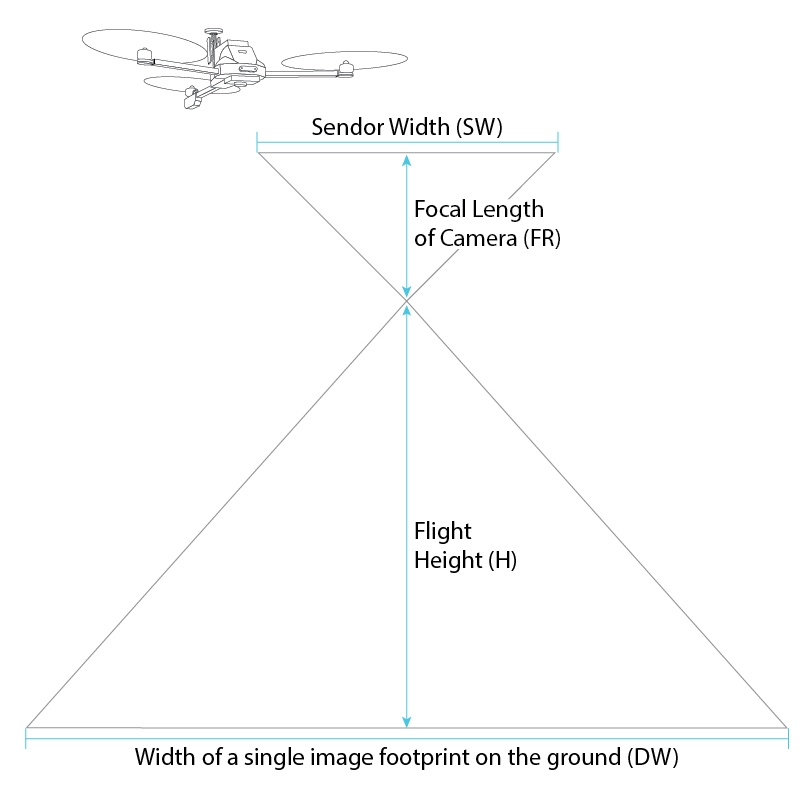
\includegraphics[width=0.5\textwidth]{images/gsd_drone_example.jpg}
    \caption{Interpretación del GSD.}
    \label{fig:gsd_example}
\end{figure}



Por tanto, para resolver la distancia real al objeto es necesario averiguar la distancia focal de la cámara. Para ello, OpenCV proporciona métodos de calibración de cámaras basados en la detección de patrones conocidos. En este proyecto se utilizó el patrón de ``ajedrez'', ilustrado en la \textbf{figura \ref{fig:patron_ajedrez}}.

Para realizar la calibración, se desarrolló un algoritmo que toma 10 imágenes del patrón y las introduce en la función \textit{cv::calibrateCamera()}, la cual devuelve tres datos: la matriz intrínseca con los valores de $F_x, F_y, C_xyC_y$, el vector de coeficientes de distorsión y, finalmente, un valor ``double'' que indica el error de calibración (rms).

Se llevaron a cabo 10 calibraciones con el mismo patrón y se seleccionaron las 4 con mejor resultado (rms $<$ 0{,}3). A partir de ellas se calculó la media aritmética de la distancia focal en los ejes $x$ e $y$, obteniendo finalmente:

$F_x \approx 1472.768 * 0.00421875 \approx 6.21 mm$

$F_y \approx 1449.567 * 0.004375 \approx 6.34 mm$

$C_x \approx 86.747 * 0.00421875 \approx 0.37 mm$

$C_y \approx 50.412 * 0.004375 \approx 0.22 mm$



\begin{figure}[h]
    \centering
    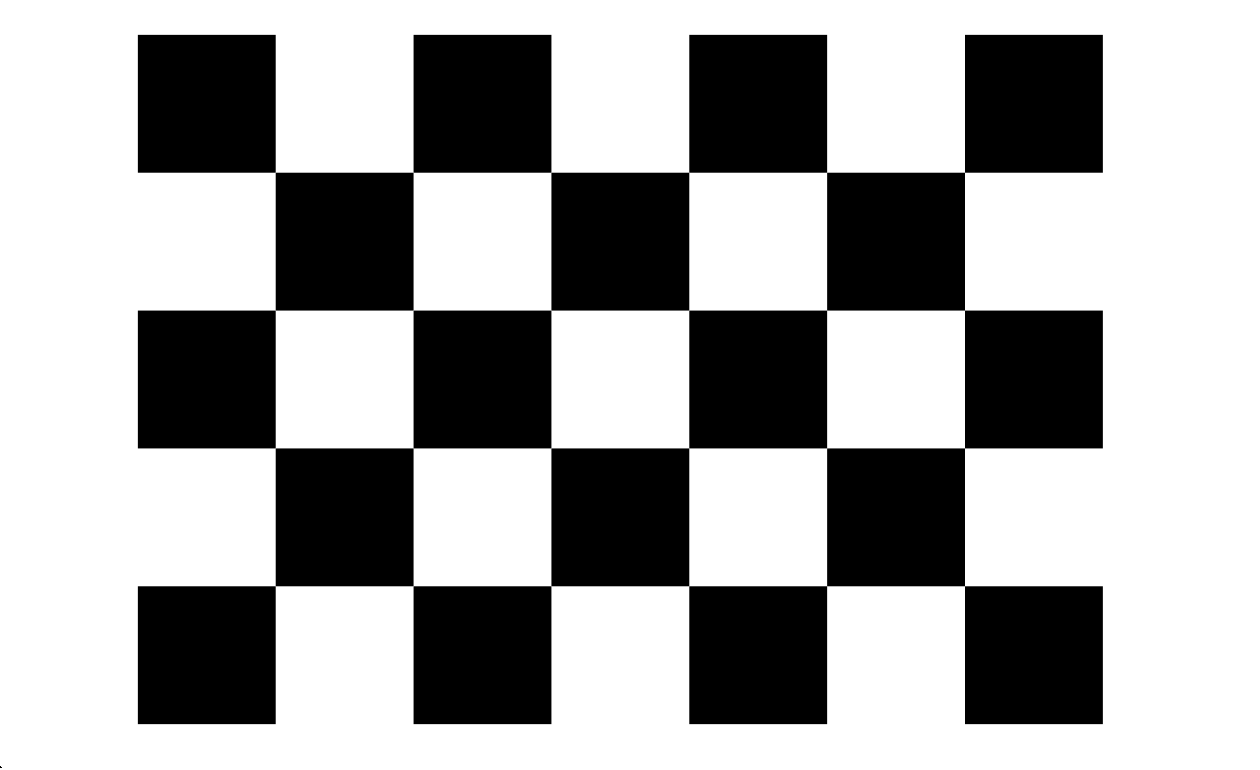
\includegraphics[width=0.7\textwidth]{images/calibracion_ajedrez.png}
    \caption{Patrón de calibración de ''ajedrez''.}
    \label{fig:patron_ajedrez}
\end{figure}


Aquí es donde entra en juego el uso del detector de objetos YOLO v11. Este detector proporciona una ``bounding box'' de las clases seleccionadas, y, guardando en un archivo \texttt{.txt} el ancho y el alto reales medios en metros de dichos objetos, es posible inferir su distancia real.

En la \textbf{figura \ref{fig:taza_extrapolacion}} se puede observar la salida de valores normalizados generada por MiDaS, entre 0 y 1 (derecha), así como su capacidad para interpolar la distancia real (izquierda). Como referencia, la taza se encontraba a 35 cm de la cámara.

Finakmente, el algoritmo de extrapolación extrapola todos los puntos de la imagen, si solo exsite un objeto detectado multiplica la salida de midas por el factor d e escala pero si dedetecta 2 o más objetos ajusta un polinomio de $n-1$ grados (3 tazas implica un polinomio de grado 2) y con el modifica los valores de la salida de midas según el polinomio.



\begin{figure}[h]
    \centering
    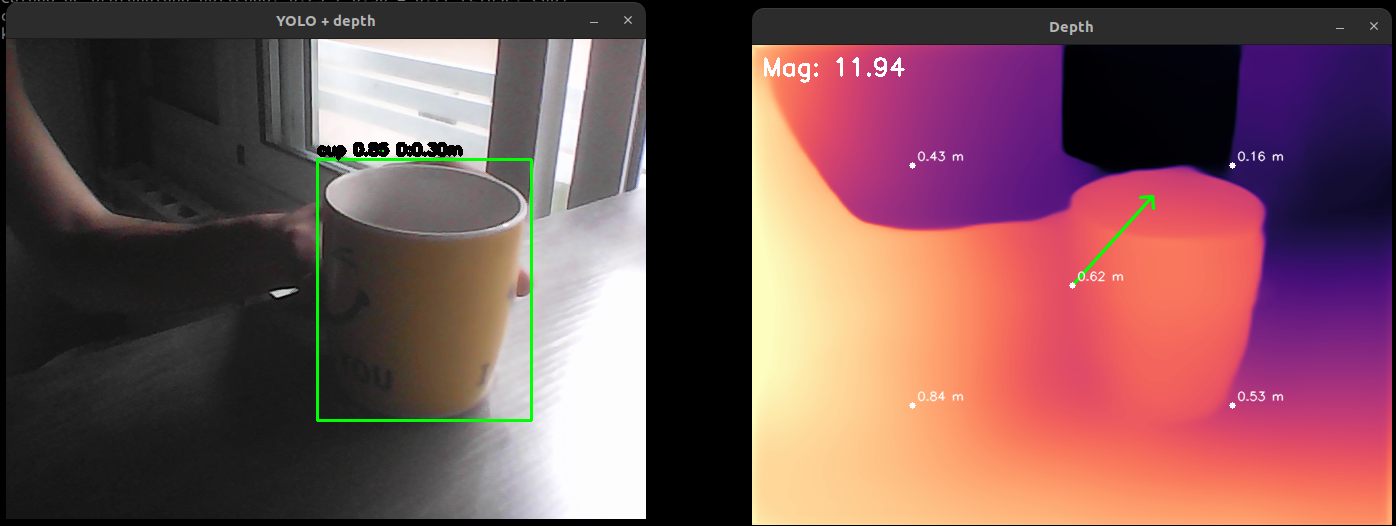
\includegraphics[width=0.9\textwidth]{images/extrapolacion_taza.png}
    \caption{Extrapolación de distancia real con una taza.}
    \label{fig:taza_extrapolacion}
\end{figure}



    % \section{Fine tuning del detector de objetos}
  \chapter{Pruebas y resultados}
En esta sección se muestran las pruebas y resultados obtenidos para cada sección del proyecto, con el objetivo de validar el correcto funcionamiento de los algoritmos desarrollados. Se incluyen capturas de pantalla, visualizaciones de salida y comparaciones cuantitativas donde corresponde.
.

    \section{Validación de la velocidad de inferencia y benchmarking del algoritmo}
Para probar y poder comparar las distintas implementaciones que se han probado en el proyecto se realizaron 6 test de performance, donde se midieron el tiempo de cada parte y el total, dando como resultado un frame rate o fps alcanzados. Todos los test se realizaron de la misma manera, primero se hizo un benchmarking del tiempo para MiDaS, YOLO y la captura de la cámara, también del total; Finalmente se realizó un profiling con la herramienta de \textit{google chrome} para visualizar los ciclos de procesamiento más en detalle. En los test se muestra una tabla con los valores y una figura con el benchamarking de cada test. 

        \subsection{Sin multi-threading, sin GPU}

\begin{table}[H]    
    \centering
    \begin{tabular}{|c|c|}
        \hline
        \textbf{Sección} & \textbf{tiempo (ms)}  \\
        \hline
        MiDaS   & 65.21     \\
        YOLO    & 94.31     \\
        Cámara  & 51.23     \\
        Total   & 210.75 (4.75 fps)   \\
        \hline
    \end{tabular}
    \caption{Tiempos para las secciones del testsin mt y sin GPU}
    \label{tab:nomt_nogpu}
\end{table}

Dado que esta implementación no usa multi-threading realizar profiling resulta innecesario.

\newpage

        \subsection{Con multi-threading, los 2 modelos en la CPU}
\begin{table}[H]
    \centering
    \begin{tabular}{|c|c|}
        \hline
        \textbf{Sección} & \textbf{tiempo (ms)}  \\
        \hline
        MiDaS   & 161,73     \\
        YOLO    & 113.28    \\
        Cámara  & 49.71   \\
        Total   & 156.32 (6.39 fps)  \\

        \hline
    \end{tabular}
    \caption{Tiempos para las secciones con los modelos en la CPU.}
    \label{tab:cpu2}
\end{table}


\begin{figure}[H]
    \centering
    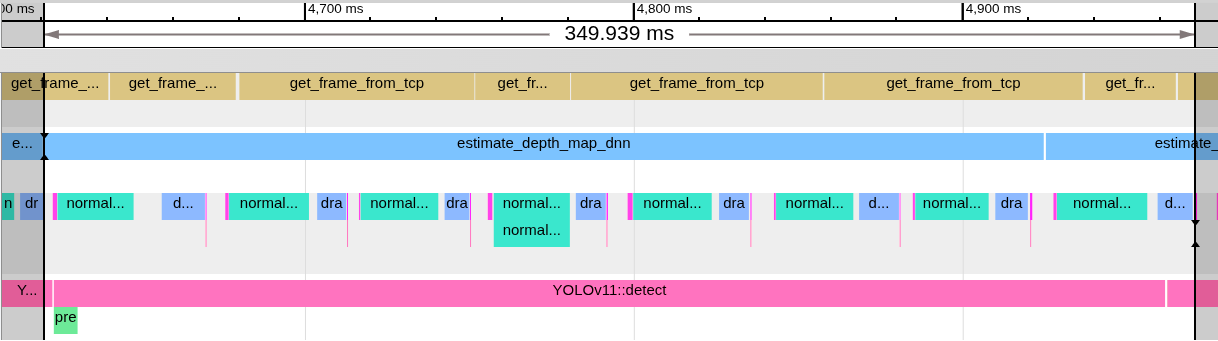
\includegraphics[width=0.7\textwidth]{images/2cpu_prof.png}
    \caption{Profiling con los modelos en la CPU.}
    \label{fig:cpu2_prof}
\end{figure}



        \subsection{Con multi-threading, los 2 modelos en la GPU}
\begin{table}[H]
    \centering
    \begin{tabular}{|c|c|}
        \hline
        \textbf{Sección} & \textbf{tiempo (ms)}  \\
        \hline
        MiDaS   & 107.03     \\
        YOLO    & 109.248    \\
        Cámara  & 49.26   \\
        Total   & 91.24 (10.96 fps)    \\

        \hline
    \end{tabular}
    \caption{Tiempos para las secciones con los modelos en la GPU.}
    \label{tab:gpu2}
\end{table}


\begin{figure}[H]
    \centering
    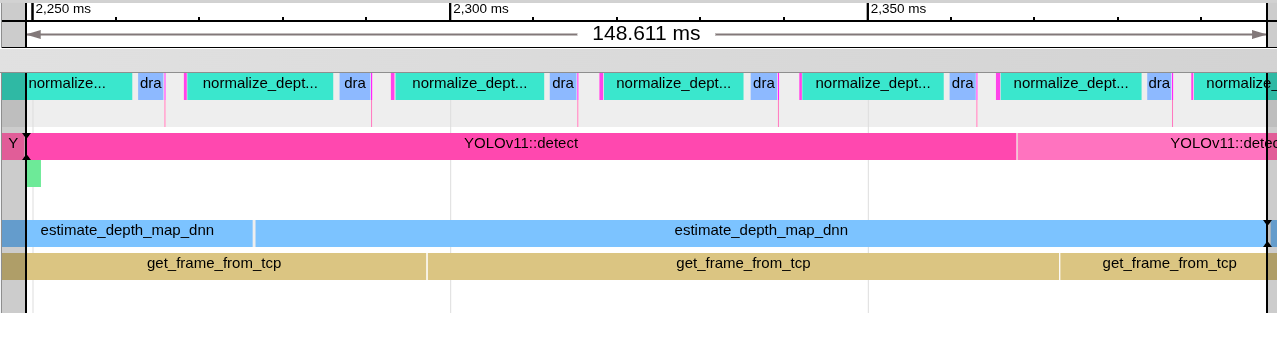
\includegraphics[width=0.7\textwidth]{images/2gpu_prof.png}
    \caption{Profiling con los modelos en la GPU.}
    \label{fig:gpu2_prof}
\end{figure}

        \subsection{Con multi-threading, YOLO en la GPU y MiDaS en la CPU}
\begin{table}[H]
    \centering
    \begin{tabular}{|c|c|}
        \hline
        \textbf{Sección} & \textbf{tiempo (ms)}  \\
        \hline
        MiDaS   & 101.03     \\
        YOLO    & 94.16    \\
        Cámara  & 53.72   \\
        Total   & 102.53 (9.75 fps)    \\

        \hline
    \end{tabular}
    \caption{Tiempos para las secciones con YOLO en la GPU y MiDaS en la CPU}
    \label{tab:yologpu_midas_cpu}
\end{table}


\begin{figure}[H]
    \centering
    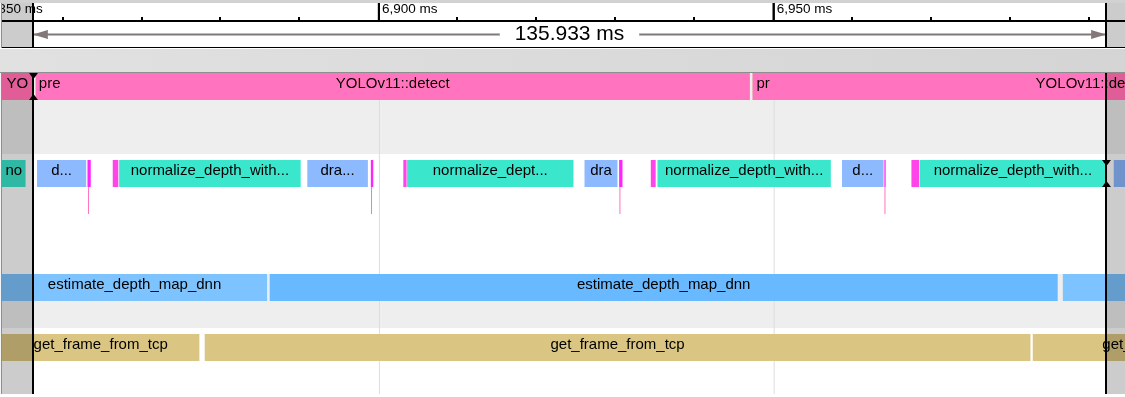
\includegraphics[width=0.7\textwidth]{images/ygpu_mcpu_prof.png}
    \caption{Profiling con YOLO en la GPU y MiDaS en la CPU.}
    \label{fig:yologpu_midas_cpu_prof}
\end{figure}



        \subsection{Con multi-threading, MiDaS en la GPU y YOLO en la CPU}
\begin{table}[H]
    \centering
    \begin{tabular}{|c|c|}
        \hline
        \textbf{Sección} & \textbf{tiempo (ms)}  \\
        \hline
        MiDaS   & 71.89     \\
        YOLO    & 75.76    \\
        Cámara  & 49.46   \\
        Total   & 67.56 (14.8 fps)    \\

        \hline
    \end{tabular}
    \caption{Tiempos para las secciones con MiDaS en la GPU y YOLO en la CPU}
    \label{tab:yolocpu_midas_gpu}
\end{table}


\begin{figure}[H]
    \centering
    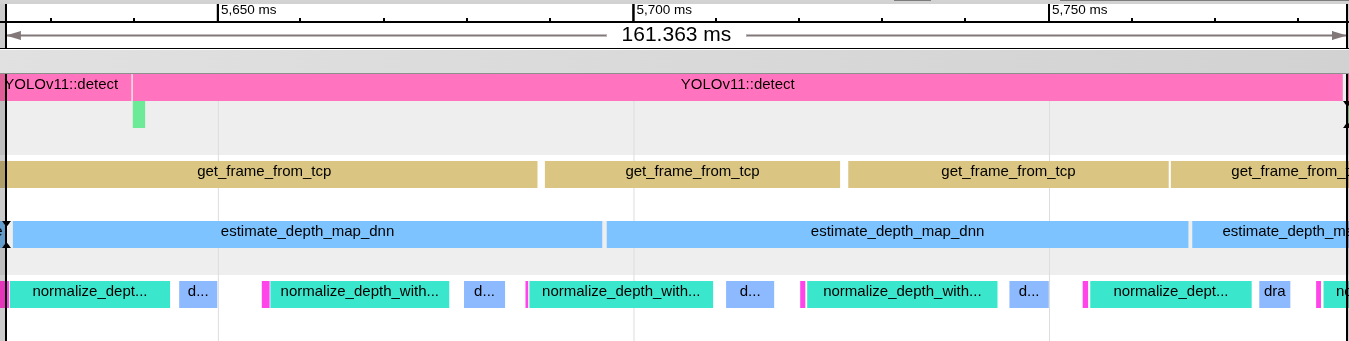
\includegraphics[width=0.7\textwidth]{images/mgpu_ycpu_prof.png}
    \caption{Profiling con MiDaS en la GPU y YOLO en la CPU.}
    \label{fig:yolocpu_midas_gpu_prof}
\end{figure}

Como se puede observar la última arquitectura es la más eficiente y rápida por lo que es la que definitivamente se usa en el trabajo, comentar también que dada la naturaleza multi-hilo del sistema y que Linux no sea un sistema \textbf{Real Time} la cuenta de ms en los diferentes test no es perfecta y tiene errores que son difícilmente solucionables, un ejemplo es el último test donde YOLO parece tardar 150 ms cuando en verdad esta tardando la mitad, de todas formas sirve como prueba y análisis de el proceso de un ciclo de procesamiento, también podemos ver como con el ''overhead'' que hemos ido añadiendo provoca que el tiempo de captura de la imagen haya subido y se mantenga  constante al rededor de los 50 ms.

    \section{Estabilización de la inferencia de profundidad}
Este experimento trata de mostrar el impacto que tiene el algoritmo de filtrado exponencial en la iamagen y además msotrar como varía la misma al variar la constante $\alpha$ de ponderación. Dada la dificultad de mostrar videos en este formato se muestran 4 frames consecutivos, donde la \textbf{figura \ref{fig:no_filter}} muestra el ''flickering'' sin filtro ninguno, aunque en el presente documento cueste ver la diferencia, en la práctica el parpadeo es extremadamente notable. En la \text{figura \ref{fig:filter_a025}} se muestra el resultado de aplicar el filtro exponencial con un $\alpha = 0.25$ siendo este el valor que proporciona el mejor resultado.

Además de estos valores se probarón también 0.1, 0.5, 0.75 y 0.98, si el valor de $\alpha$ es muy grande el filtro se ''fia'' demasiado en la salida directa de MiDaS y por tanto parpadeá con mayor intensidad, en cambio si el valor es muy bajo no ponderá bien entre 2 frames y por tanto también pierde eficacia.

\begin{figure}[H]
    \centering
    \begin{subfigure}[b]{0.45\textwidth}
        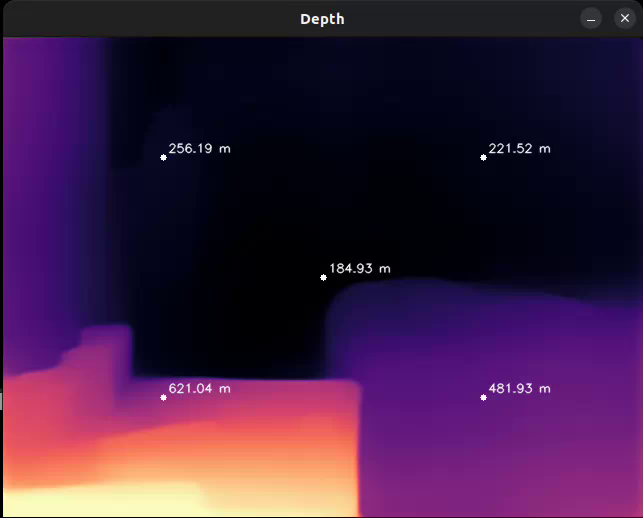
\includegraphics[width=\textwidth]{images/no_filter/frame_00000.png}
    \end{subfigure}
    \hfill
    \begin{subfigure}[b]{0.45\textwidth}
        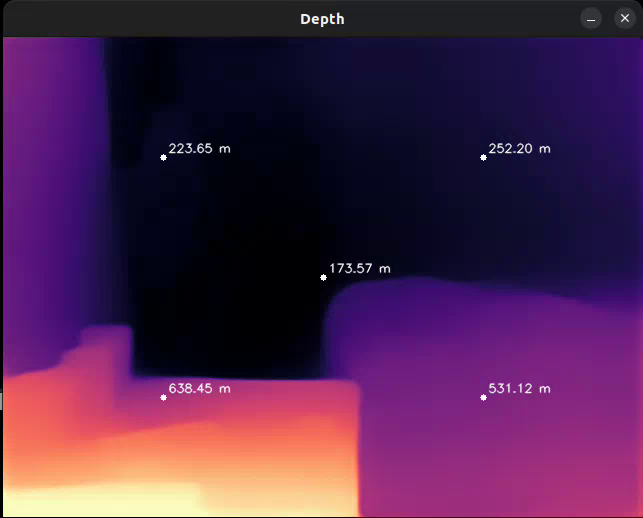
\includegraphics[width=\textwidth]{images/no_filter/frame_00008.png}
    \end{subfigure}
    \vspace{0.5cm}
    \begin{subfigure}[b]{0.45\textwidth}
        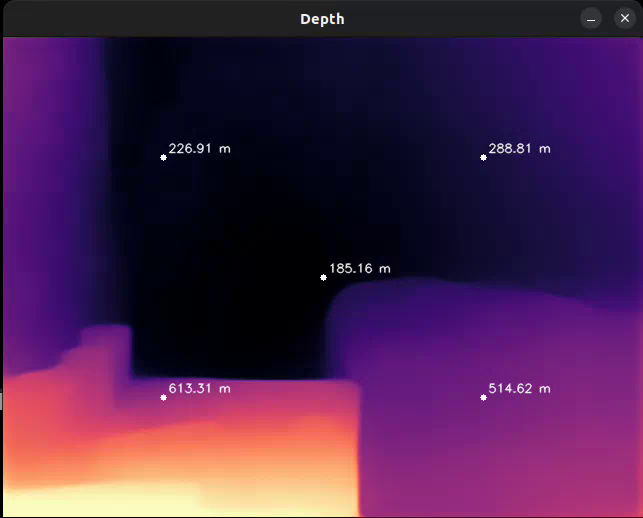
\includegraphics[width=\textwidth]{images/no_filter/frame_00016.png}
    \end{subfigure}
    \hfill
    \begin{subfigure}[b]{0.45\textwidth}
        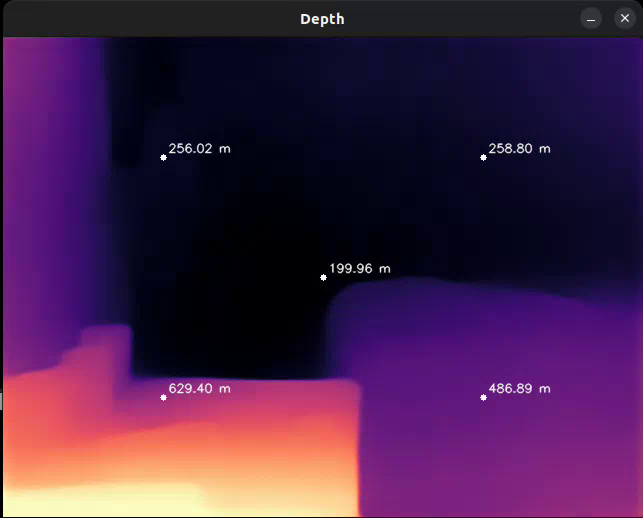
\includegraphics[width=\textwidth]{images/no_filter/frame_00022.png}
    \end{subfigure}

    \caption{Muestra de ''flickering'' sin filtro (frames 1 a 4).}
    \label{fig:no_filter}
\end{figure}

\begin{figure}[H]
    \centering
    \begin{subfigure}[b]{0.45\textwidth}
        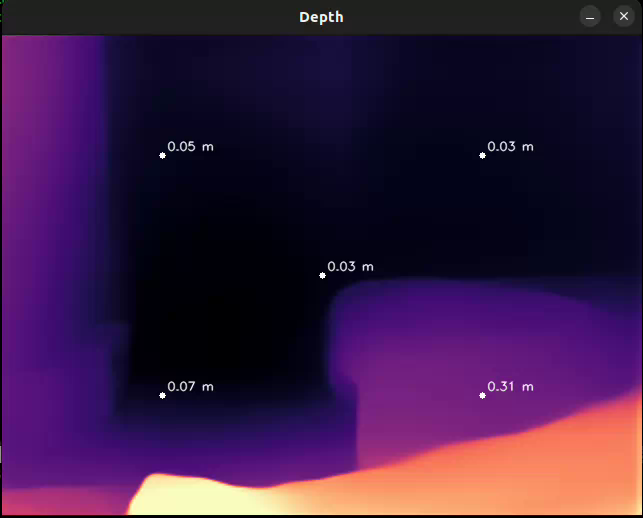
\includegraphics[width=\textwidth]{images/filter_a025/frame_00000.png}
    \end{subfigure}
    \hfill
    \begin{subfigure}[b]{0.45\textwidth}
        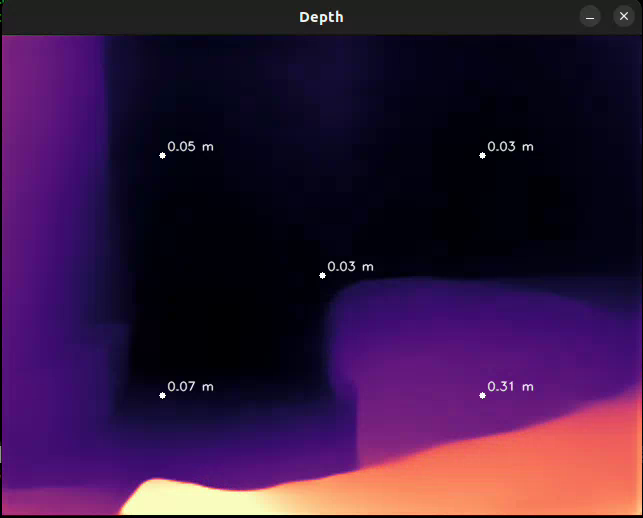
\includegraphics[width=\textwidth]{images/filter_a025/frame_00008.png}
    \end{subfigure}
    \vspace{0.5cm}
    \begin{subfigure}[b]{0.45\textwidth}
        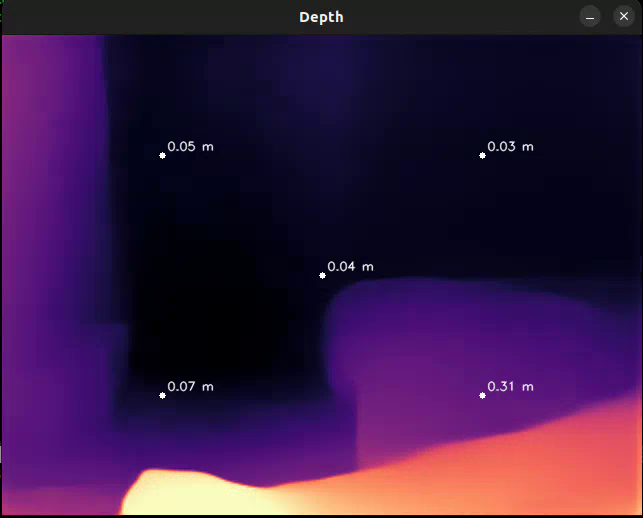
\includegraphics[width=\textwidth]{images/filter_a025/frame_00016.png}
    \end{subfigure}
    \hfill
    \begin{subfigure}[b]{0.45\textwidth}
        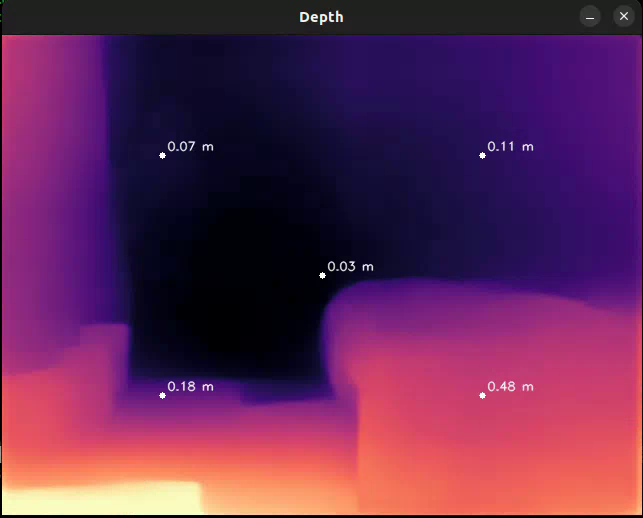
\includegraphics[width=\textwidth]{images/filter_a025/frame_00024.png}
    \end{subfigure}

    \caption{Muestra de ''flickering'' con filtro  y alpha = 0.25(frames 1 a 4).}
    \label{fig:filter_a025}
\end{figure}
    \section{Pruebas de interpolación de distancias}
Para este test se evaluó la precisión del algoritmo de interpolación de distancias utilizando 0, 1 y 2 objetos detectados. La prueba se realizó únicamente con una clase conocida (una taza) a la que se le añadió un archivo \textit{.txt} con su información real de ancho y alto en metros, con el siguiente formato: \textit{cup 0.08 0.12}, donde \texttt{0.08} corresponde al ancho y \texttt{0.12} a la altura, ambos en metros.

A continuación se presentan cuatro imágenes que ilustran el correcto funcionamiento del sistema. La \textbf{figura \ref{fig:setup_inter}} muestra el "setup" experimental, donde se puede observar un metro físico para comparar la distancia real con la estimada por el algoritmo. La cámara se colocó pegada a la pared para simular una visión horizontal de la escena, y las tazas se fueron posicionando a distintas distancias no uniformes.

\begin{figure}[H]
\centering
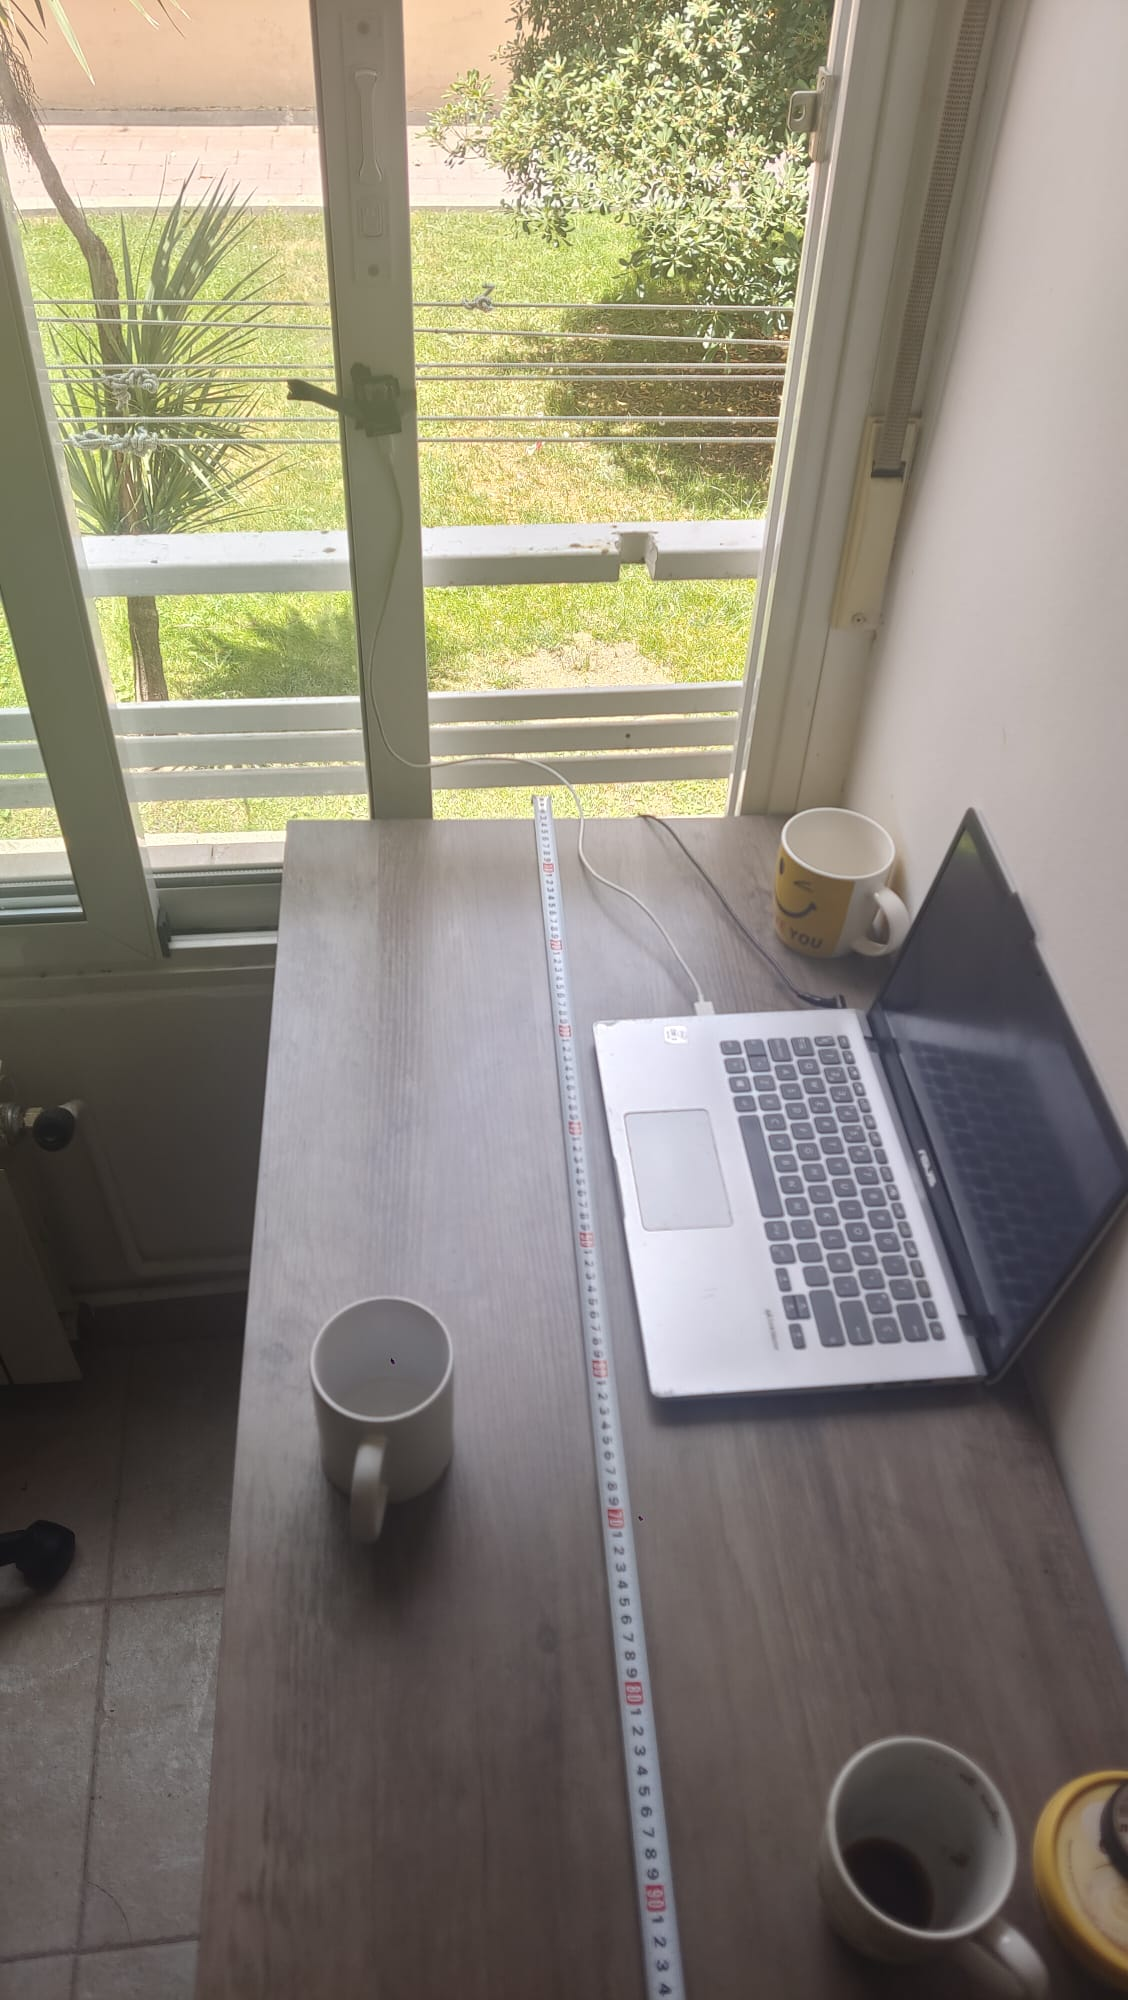
\includegraphics[width=0.4\textwidth,angle=90]{images/setup_inter.jpeg}
\caption{Setup para el experimento de interpolación de distancias.}
\label{fig:setup_inter}
\end{figure}

La \textbf{figura \ref{fig:0obj_inter}} sirve como imagen de control del experimento. En ella se muestra el resultado del algoritmo cuando no se detecta ningún objeto. Como es de esperar, los valores de profundidad se encuentran entre 0 y 1, lo cual confirma el comportamiento normal del sistema en ausencia de datos de referencia.

\begin{figure}[H]
\centering
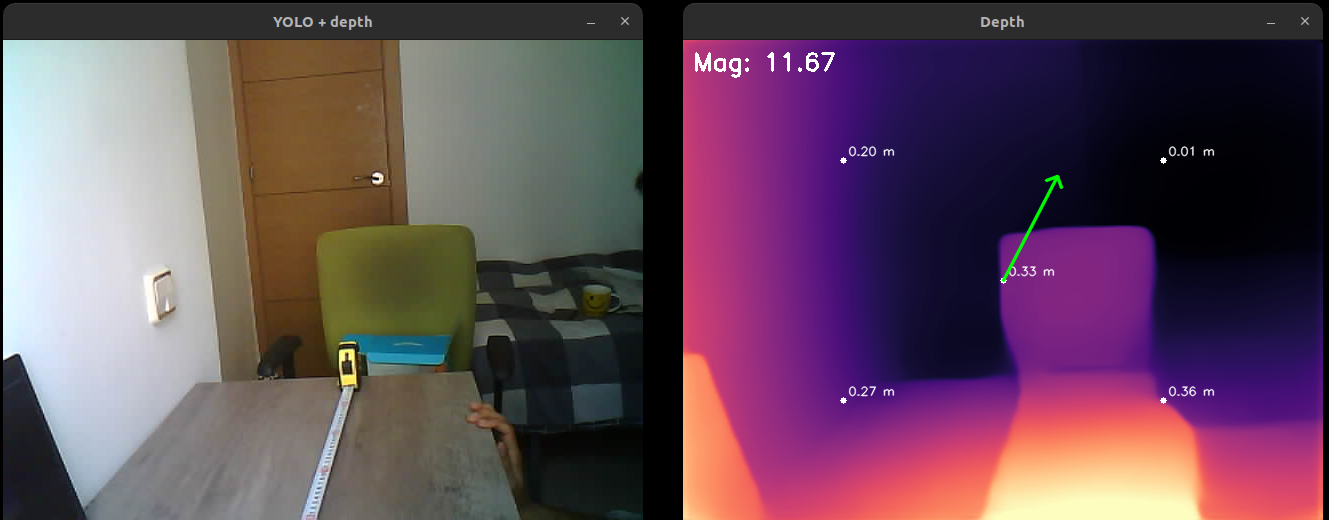
\includegraphics[width=0.8\textwidth]{images/0objetos_interpolacion.png}
\caption{Interpolación de distancias sin objetos (imagen de control).}
\label{fig:0obj_inter}
\end{figure}

En la \textbf{figura \ref{fig:1obj_inter}} se observa cómo el sistema estima las distancias cuando se detecta un solo objeto. El algoritmo ofrece buenos resultados en las proximidades del objeto detectado, pero pierde precisión a medida que se aleja. Por ejemplo, el punto en el primer cuadrante indica 32 metros cuando, en realidad, la pared se encuentra a 2.6 metros. Como referencia, la taza estaba situada a exactamente 0.77 m y la silla a 1.8 m del sensor de la cámara.

\begin{figure}[H]
\centering
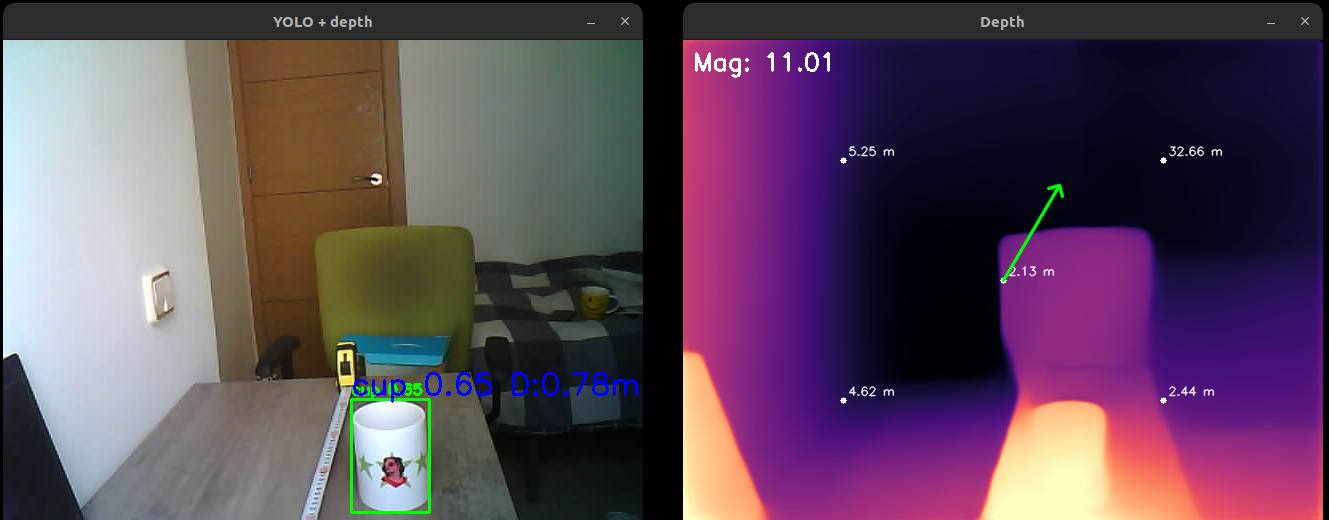
\includegraphics[width=0.8\textwidth]{images/1objetos_interpolacion.png}
\caption{Interpolación de distancias con 1 objeto.}
\label{fig:1obj_inter}
\end{figure}

En la \textbf{figura \ref{fig:2obj_inter}} se muestra el resultado con 2 objetos detectados. Aquí la salida mejora significativamente: la taza sobre la silla se estima a exactamente 1.86 m y la pared del fondo, que antes se estimaba a 32 m, ahora aparece a 2.41 m. Considerando que la distancia real es de 2.6 m, esto representa un error de apenas 20 cm.

\begin{figure}[H]
\centering
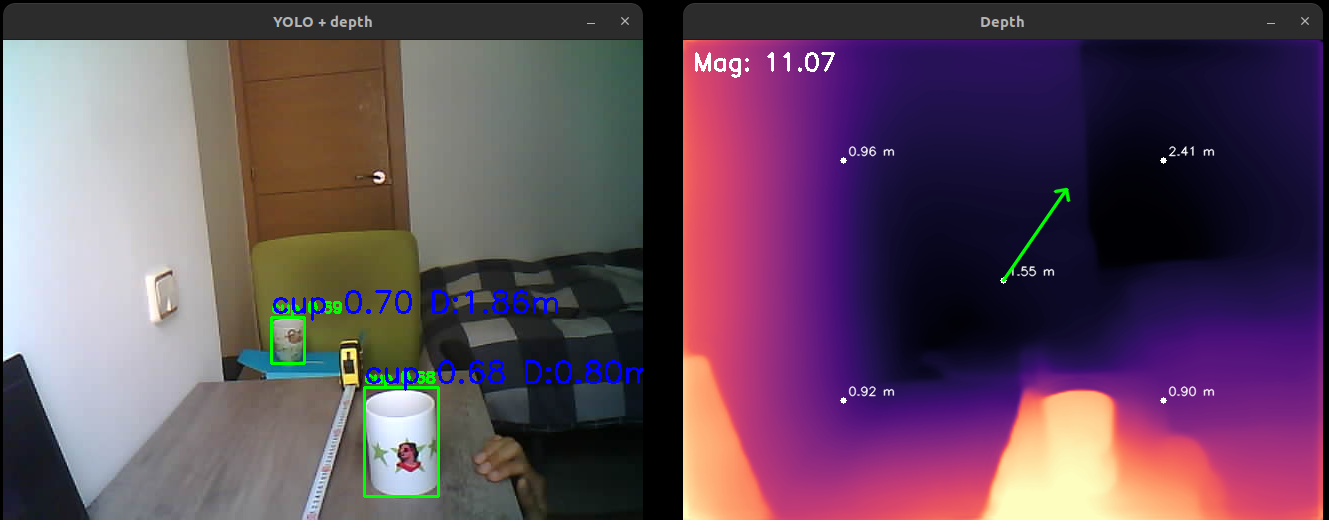
\includegraphics[width=0.8\textwidth]{images/2objetos_interpolacion.png}
\caption{Interpolación de distancias con 2 objetos.}
\label{fig:2obj_inter}
\end{figure}

Del desarrollo del test se pueden extraer varias conclusiones. En primer lugar, el algoritmo logra estimar con un error moderado la distancia real de los objetos en la escena. Sin embargo, presenta ciertas limitaciones. Una de ellas es la dificultad para interpolar correctamente cuando los objetos detectados están muy cerca entre sí, lo cual restringe la interpolación a su vecindad inmediata, como si solo se hubiera detectado un objeto. Otra dificultad importante surge al intentar estimar la profundidad de objetos pequeños situados a gran distancia, ya que estos tienden a no ser detectados. Esto sugiere que, en el futuro, será necesario emplear objetos lo suficientemente grandes para que puedan ser detectados a larga distancia y así obtener una mejor estimación global de la profundidad.

Por último, se identificó una limitación técnica relacionada con el sobrecalentamiento tanto del ordenador como de la cámara, lo cual provoca ralentizaciones, bloqueos temporales en la transmisión de frames y una disminución en la capacidad de detección múltiple.

  \chapter{Conclusiones y lineas futuras}

El proyecto ha logrado desarrollar un método fiable, robusto y lo suficientemente rápido como para ser ejecutado en tiempo real. Los resultados de velocidad muestran valores muy cercanos al \textit{frame rate} máximo teórico, determinado por la velocidad de la cámara. Se ha conseguido desarrollar una arquitectura de software estable tanto ante cambios en la iluminación o la posición, como frente al ``flickering'' intrínseco del modelo estimador de profundidad.

El algoritmo de extrapolación de distancia ha sido probado extensamente y presenta un error menor a 40 cm para un número  mayor a 2 detecciones y en el rango de metros para solo 1 objeto.

En general, aunque aún existen múltiples posibilidades de mejora, se ha demostrado que el presente proyecto tiene un gran potencial para convertirse en un algoritmo robusto y viable para su uso en drones de bajo coste y con una velocidad moderada de movimiento.

Como líneas futuras, se plantean:

\begin{itemize}
\item Realizar \textit{fine-tuning} con YOLO para detectar únicamente objetos estáticos y visibles en entornos exteriores, también que objetos que sea viable ''ver'' tanto por sus semántica como por su tamaño.
\item Ajustar el sistema para mejorar aún más la precisión en la extrapolación de distancias, perfeccionando la calibración de la cámara y haciendo el algoritmo más robusto frente a excepciones.
\item Refinar los algoritmos de normalización y filtrado exponencial para aumentar la robustez general.
\item Aplicar otros métodos de visión, como HOG, para la búsqueda de direcciones de movimiento.
\item Desarrollar un algoritmo que permita mantener la distancia estimada de los objetos, incluso cuando no sean detectados por YOLO.
\end{itemize}

    